  
     %%%%%%%%%%%%%%%%%%%%
     %                  %
     %  capitolo4.tex   %
     %                  %
     %%%%%%%%%%%%%%%%%%%%

\chapter{Some analysis of the fixed point equations}
\noindent
The quest for \emph{fixed points} is essential in any RG-based theory: in quantum field theory, the fixed points structure determine also the nature of the continuum limit and as in statistical physics their nature let control the large distance behavior at criticality.

In the large $N$ limit of the $O(N)$ model, the fixed points are defined as the solutions of the system:
\begin{equation}
\label{sistema}
\left\{
\begin{array}{l}
\dot{w}_k(\widetilde{\rho}) = 0\\
\dot{z}_k(\widetilde{\rho}) = 0\\
\end{array}
\right.
\end{equation}
In this chapter I will start to study the fixed point structure of the $O(N)$ model in the large $N$ limit, in $D=3$ and $D=5$, analyzing the behavior of the derivative of the dimensionless effective potential $w_k(\rho)$ and of the wavefunction renormalization $z_k(\rho)$ in those points, using the
flow equations \eqref{wpuntolargeN} and \eqref{zpuntolargeN} derived in the previous chapter of this thesis. I will distinguish 
between three different situations:

\begin{enumerate}
 \item $\eta_k = 0$ and $z'_k(\widetilde{\rho}) = 0$, already completely studied (see, for example, \cite{vaccascaling}).
 \item $\eta_k \neq 0$ and $z'_k(\widetilde{\rho}) \neq 0$
 \item $\eta_k = 0$ and $z'_k(\widetilde{\rho}) \neq 0$
\end{enumerate}
As I will show, for the first of those cases, analytical exact solutions are available.

In the following I will choose as regulator the \emph{Litim optimized regulator}, discussed in the second chapter of this thesis:
\begin{equation}
R_k(q^2) = Z_k(k^2 - q^2)\theta(k^2 - q^2)
\end{equation}
So, the renormalized one is:
\begin{equation}
{r}_k(y) = \left(\frac{1}{y} - 1\right)\theta(1-y)
\end{equation}
With that choice, the system \eqref{sistema} becomes:
\begin{equation}
\left\{
\begin{array}{l}
(\eta_k -2 )w_k(\widetilde{\rho}) + (D-2 +\eta_k)\widetilde{\rho}\frac{\partial w_k(\widetilde{\rho})}{\partial \widetilde{\rho}} - v_D\int_0^1 dy \frac{y^{\frac{D}{2}-1}    (2-\eta_k + \eta_ky)(z'_k(\widetilde{\rho})y + w'_k(\widetilde{\rho}))}{\big([z_k(\widetilde{\rho}) -1 ]y  +  w_k(\widetilde{\rho})+ 1\big)^2} = 0\\
\eta z_k(\widetilde{\rho}) + (D-2+\eta)\widetilde{\rho}\frac{\partial z_k(\widetilde{\rho})}{\partial \widetilde{\rho}}  -v_D\int_0^1 dy \frac{y^{\frac{D}{2}-1}  (2-\eta_k + \eta_ky) z'_k(\widetilde{\rho})}{\big([z_k(\widetilde{\rho}) -1 ]y  +  w_k(\widetilde{\rho})+ 1\big)^2} = 0
\end{array}
\right.
\end{equation}
For the sake of completeness, I also report the large $N$ limit of the flow equation of the dimensionless effective potential, with our choice of the regulator:
\begin{equation}
 \dot{u}_k(\widetilde{\rho}) = -D  u_k(\widetilde{\rho}) +(D - 2 + \eta)\widetilde{\rho}\frac{\partial u_k(\widetilde{\rho})}{\partial \widetilde{\rho}} - v_D \int_0^\infty  \frac{y^{\frac{D}{2}-1}  (2-\eta_k + \eta_ky) }{y[z_k(\widetilde{\rho}) + r_k(y)] + u_k'(\widetilde{\rho})} dy 
\end{equation}

\section{First case: $\eta_k = 0$ and $z'_k(\rho)= 0$}
If $z_k(\widetilde{\rho})$ is a constant function both of the field strength and of $k$ (the latter is equivalent to the 
requirement of a vanishing anomalous dimension), the flow equation for the renormalized potential \eqref{upuntolargeN} can be solved
in an analytically closed form\cite{1}\cite{12}\cite{13}.

Because of the conditions $\dot{z}_k(\widetilde{\rho}) = 0$ and $z'_k(\widetilde{\rho}) = 0$, we have ${z}_k(\widetilde{\rho}) = 1$, so the system \eqref{sistema} reduces to the single equation:

\begin{equation*}
-2 w_k(\widetilde{\rho}) + (D-2)\widetilde{\rho}\frac{\partial w_k(\widetilde{\rho})}{\partial \widetilde{\rho}} - 2v_D\int_0^1 dy \frac{y^{\frac{D}{2}-1} w'_k(\widetilde{\rho})}{\big([z_k(\widetilde{\rho}) -1 ]y + w_k(\widetilde{\rho})+1\big)^2}  = 
\end{equation*}
\begin{equation}\label{wcase1}
 = -2 w_k(\widetilde{\rho}) + (D-2)\widetilde{\rho}w'_k(\widetilde{\rho}) - \frac{4v_D}{D} \frac{w'_k(\widetilde{\rho})}{\big(w_k(\widetilde{\rho})+1\big)^2}=0
\end{equation}

\subsection{Asymptotic behavior}
In this section I want to study the asymptotic behavior of our system or, in other words, its behavior for $\rho \to \infty$. 

It is easy to see that in this limit the nonlinear differential equation constraints usually the effective potential $u_k(\widetilde{\rho})$ and its derivative $w_k(\widetilde{\rho})$ 
to go to infinity so that the last term in the eq.\eqref{wcase1} is suppressed with respect to the other ones. This happens, for example, 
for the Wilson-Fisher scaling solution for $D= 3$. In general one can write a full asymptotical expansion for the solution.

In order to estract the leading behavior, we can rewrite the large fields limit of eq.\eqref{wcase1} obtaining:
\begin{equation}\label{wasi}
-2 w_k(\widetilde{\rho}) + (D-2)\widetilde{\rho} w'_k(\widetilde{\rho}) = 0
\end{equation}
This equation can be easily integrated giving the following result for the asymptotic behavior of $ w_k(\widetilde{\rho})$:
\begin{equation}\label{wasi}
w_k(\widetilde{\rho}) \approx A \widetilde{\rho}^{\frac{2}{D -2}}
\end{equation}
At last, the asymptotic behavior of the effective potential is recovered integrating this equation with respect to $\widetilde{\rho}$:
\begin{equation}
u_k(\widetilde{\rho}) \approx A' \widetilde{\rho}^{\frac{D}{D -2}}
\end{equation}
One can sistematically compute the subleading term of the asymptotic expansion in powers of $\widetilde{\rho}$.
For example, in $D=3$ the first terms have been calculated and they read:
\begin{equation}
\frac{1}{15 A \rho ^2}-\frac{1}{63 A^2 \rho ^4}+\frac{1}{243 A^3 \rho^6}-\frac{1}{891 A^4 \rho ^8}+\frac{1}{3159 A^5 \rho ^{10}}+\frac{4}{91125 A^5 \rho ^{12}}-\frac{1}{10935 A^6 \rho ^{12}} + \dots 
\end{equation}

\subsection{Fixed points}

A first trivial solution of the fixed point equation \eqref{wcase1} is the so called \emph{Gaussian fixed point}, that is the configuration of a constant potential:
\begin{equation}
 u_k(\widetilde{\rho}) = const\ \ \ \Longrightarrow u'_k(\widetilde{\rho}) = w_k(\widetilde{\rho}) = 0 
\end{equation}

The other, non trivial, solution is found integrating analytically equation \eqref{wcase1} (see, for example, ref. \cite{Marchais}\cite{vaccascaling}).

Here  I will just state the final result.
The solution is expressed in an implicit form, as $ \widetilde{\rho}(w)$ and it reads:
\begin{equation}\label{vacca1}
 \widetilde{\rho}(w) = C' w^{\frac{D}{2} - 1} + \frac{1}{(d + 2)(1 + w)^2} \ _2F_1\left(1, 2, 2 + \frac{D}{2}, \frac{1}{1 + w}\right)
\end{equation}
where $C'$ is an integration constant.
The special function appearing in the fixed point equation \eqref{vacca1} is the \emph{Gauss's Hypergeometric function}, defined by the series expansion \cite{M117}\cite{M118}:
\begin{equation}\label{serieiper}
 \ _2F_1\left(a, b, c, z\right) = \frac{\Gamma(c)}{\Gamma(a)\Gamma(b)}\sum_{n = 0}^{\infty} \frac{\Gamma(a + n)\Gamma(b + n)}{\Gamma(c + n)}\frac{z^n}{n!}
\end{equation}
on the disc $|z| < 1$ and by analytic continuation elsewhere. In addition to that, the serie representation \eqref{serieiper} becomes meaningless  for negative (or zero) 
values of the parameter $c$.
For values of $D$ different from even integers, the fixed points equation \eqref{vacca1} can be written in the most convenient way:
\begin{equation}\label{vacca2}
  \widetilde{\rho}(w) = C w^{\frac{D}{2} - 1} + \frac{1}{(d + 2)} \ _2F_1\left(2, 1 - \frac{D}{2}, 2 - \frac{D}{2}, -w \right)
\end{equation}
where $C' = C - \frac{D\pi}{4 \sin(D\pi/2)}$. The only real solution of equation \eqref{vacca2} that can be extended continuously through $w = 0$
is the one with $C = 0$, which represents what in the literature is called the \emph{Wilson-Fisher fixed point}.
The plots of $w(\widetilde{\rho})$ at the nontrivial fixed point for $D= 3$ and $D=5$ are reported in Fig.\ref{fig:potenziali}.

Note that in $D=5$ the potential is not defined everywhere and there is no physical solution.

%%RICOPIARE ARTICOLO VACCA
\begin{figure}
\begin{center}
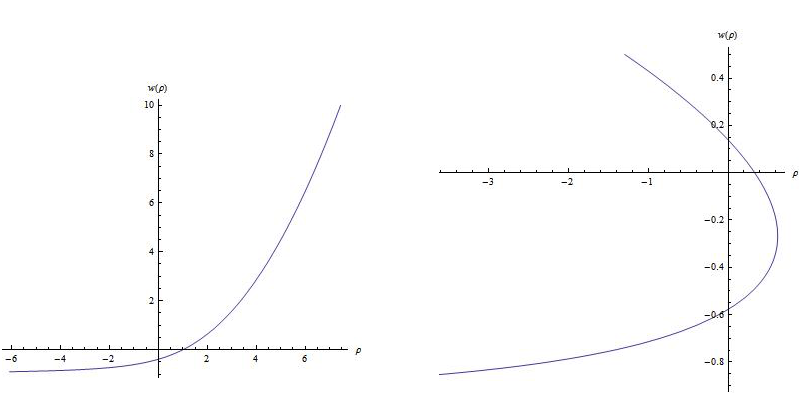
\includegraphics[scale=0.35]{Immagini/potenziali.png}
\caption{A plot of the scaling dimensionless derivative of the potential for $N\to\infty$ in $D=3$ (left) and $D=5$ (right) for $C = 0$ and the optimised Litim regulator.}
\label{fig:potenziali}
\end{center}
\end{figure}
\section{Second case: $\eta_k \neq 0$ and $z'_k(\rho) \neq 0$}
The second case I am going to study is also the most general one, the case of a non constant wavefunction renormalization and of a non vanishing anomalous dimension.
First of all, in order to simplify the notations, I will state some definitions and I will expose the results of some integrals that will be useful in the following.
\subsection{Integrals}
In order to study the flow equations in the most general case, we need to know the explicit expressions of the integrals:
\begin{equation}\label{4ediciotto}
\Int(\alpha) = \int_0^1 dy \frac{y^{\frac{\alpha}{2}}}{\big([z_k(\widetilde{\rho}) -1 ]y  +  w_k(\widetilde{\rho})+ 1\big)^2}
\end{equation}
Because we are interested in the behavior of the model in $D =3$ and in $D=5$, recalling the expressions of the flow equations \eqref{SEDICI},
we need to calculate the following integrals:
\begin{equation}\label{D1}
\Int(1) = - \frac{\tanh ^{-1}\left(\sqrt{\frac{1-z}{w+1}}\right)}{(w+1)^{1/2} (1-z)^{3/2}}+ \frac{1}{(1-z) (w+z)}
\end{equation}
\begin{equation}\label{D3}
\Int(3) = \frac{3 w+2 z+1}{(z-1)^2 (w+z)}-\frac{3 \sqrt{w+1} \tanh ^{-1}\left(\sqrt{\frac{1-z}{w+1}}\right)}{(1-z)^{5/2}}
\end{equation}
\begin{equation}\label{D5}
\Int(5) = \frac{15 w^2+10 w (z+2)-2 (z-7) z+3}{3 (1-z)^3 (w+z)}-\frac{5 (w+1)^{3/2} \tanh ^{-1}\left(\sqrt{\frac{1-z}{w+1}}\right)}{(1-z)^{7/2}}
\end{equation} 
\begin{equation}\label{D7}
\Int(7) = \frac{105 w^3+35 w^2 (2 z+7)-7 w \left(2 z^2-24 z-23\right)+6 z^3-32 z^2+116 z+15}{15 (z-1)^4 (w+z)}-
\end{equation}
\begin{equation*}
 - \frac{7 (w+1)^{5/2} \tanh ^{-1}\left(\sqrt{\frac{1-z}{w+1}}\right)}{(1-z)^{9/2}}
\end{equation*}
Where all the previous solution have validity range $w + z \geq 0$.

Here and in the following, in order to lighten the notations, I have indicated $\widetilde{\rho}$, $w_k(\widetilde{\rho})$, $ z_k(\widetilde{\rho})$ and $\eta_k$  simply with ${\rho}$, $w$, $z$ and $\eta$ respectively.

\subsection{The exact equations}
Now we have all the elements we need in order to write in an useful form the equations:
\begin{equation}\label{SEDICI}
\left\{
\begin{array}{l}
 (\eta -2)w + (D -2 +\eta){\rho} w' - v_D \Big[(2-\eta)w'\Int(D-2) + \big((2-\eta)z' + \eta w'\big)\Int(D) + \eta z'\Int(D + 2)\Big] = 0\\
\eta {z} + (1+\eta)\rho z'  - v_D {z'} \left[(2 - \eta)\Int(D-2) + \eta \Int(D)\right] = 0\\
\end{array}
\right.
\end{equation}
\subsection{Asymptotic behavior}
\subsubsection{Leading order}
In the large field limit, ${\rho} \to \infty$, the second equation of the system \eqref{SEDICI} reduces to:
\begin{equation}
 \eta_k {z({\rho})} + (D-2+\eta){\rho}{z'({\rho})} = 0
\end{equation}
And, by integration, we come to the asymptotic behavior of $z_k$:
\begin{equation}\label{427}
 z({\rho}) \approx B{\rho}^{\frac{-\eta}{D-2+\eta}}
\end{equation}
Where $B$ is an integration constant.
Now, knowing the behavior of $z$ (and, consequently, of $z'$), we can easily see that the integral in the first equation of the system \eqref{SEDICI} becomes 
negligible with respect to the others, so the equation assumes the simplified form:
\begin{equation}
(\eta -2 )w({\rho}) + (D-2 +\eta){\rho} w'({\rho})=0
\end{equation}
at the end we come, after a trivial integration, to the following result:
\begin{equation}\label{429}
w({\rho}) \approx A{\rho}^\frac{2 - \eta}{D - 2 + \eta}
\end{equation}
where $A$ is the integration constant. 
Integrating this with respect to $\rho$, we obtain the asymptotic behavior of the effective potential:
\begin{equation}
u({\rho}) \approx A\frac{D-2+\eta}{D}{\rho}^\frac{D}{D - 2 + \eta}
\end{equation}
In the limit of a vanishing anomalous dimension we note that the results found in the previous section for $u_k$ and $w_k$ are recovered. 
\subsubsection{Next to leading order}
In order to go beyond the leading order (classical) approximations \eqref{427} and \eqref{429}, I had evaluated the first non zero terms in the 
integrals we see in the system \eqref{SEDICI}. 

We know, assuming that $0<\eta<1$, $D>3$ and taking into account the classical solutions just derived in the previous paragraph, that the integrands
of the functions $\Int(\alpha)$ defined in \eqref{4ediciotto} can be approximated, at the leading order, in a neighborhood of the infinity, as:
\begin{equation}
\frac{1}{([z-1]+1+w)^2} \approx \left.\frac{1}{w^2}\right|_{w = A{\rho}^\frac{2 - \eta}{D - 2 + \eta}} + O\big(\rho^{\frac{D-2+\eta}{2(2-\eta)}}\big)
\end{equation}
Now, considering that $z'$ is suppressed with respect to $w'$, the leading corection in the first equation of the system \eqref{SEDICI} is:
\begin{equation}
 v_D\int_0^1 \frac{w'}{w^2} y^{\frac{D}{2}-1} (2-\eta +\eta  y)dy
\end{equation}
so, substituting the leading order expression for $w$ \eqref{429} and its derivative $w'$, we come to the result:
\begin{equation}
 \rho  (D-2 +\eta) w'(\rho )+(\eta -2) w(\rho )=-\frac{v_D \left(4 (\eta -2) (D-\eta +2) \rho ^{-\frac{D}{D+\eta -2}}\right)}{A D (D+2) (D -2 +\eta )}
\end{equation}
and, finally, we come to the next-to-leading order term in $w$:
\begin{equation}
 w(\rho) \approx A \rho ^{\frac{D}{D-2 +\eta}-1}+\frac{ (\eta -2) \rho ^{-\frac{D}{D-2+\eta}}}{A 2^{D+1} \pi ^{\frac{D}{2}}(D-2+\eta) \Gamma \left(\frac{D}{2}+2\right)}
\end{equation}
The first correction to the fixed point equation for $z$ can be derived in a very similar way. We have:
\begin{equation}
 \eta z_k(\widetilde{\rho}) + (D-2+\eta)\widetilde{\rho}z'_k(\widetilde{\rho})  -v_D\int_0^1 \frac{z'}{w^2} y^{\frac{D}{2}-1} (2-\eta +\eta  y)dy = 0
\end{equation}
Substituting the leading order expression of $w$ and $z'$ in the integral and integrating in $y$ we obtain:
\begin{equation}
 \rho  (D -2+\eta) z'(\rho )+\eta  z(\rho )= -\frac{v_D \left(4 B \eta  (D-\eta +2) \rho ^{-\frac{D+2}{D -2+\eta}}\right)}{A^2 D (D+2) (D-2+\eta)}
\end{equation}
this ordinary differential equation can be easily integrated, giving the result:
\begin{equation}
 z(\rho) \approx  B \rho ^{-\frac{\eta }{D+\eta -2}} \left(1+\frac{ \eta  \rho ^{1-\frac{2D}{D+\eta -2}}}{A^22^{D+1} \pi ^{\frac{D}{2}}(D -2+\eta) \Gamma \left(\frac{D}{2}+2\right)}\right)
\end{equation}

\subsection{Equations in $D=3$}
In $D=3$, recalling that $v_3 = (8\pi^2)^{-1}$, the system \eqref{SEDICI} reduces to:
\begin{equation}
\left\{
\begin{array}{l}
 (\eta -2)w + (1 +\eta){\rho} w' - \frac{1}{8\pi^2}\Big[(2-\eta)w'\Int(1) + \big((2-\eta)z' + \eta w'\big)\Int(3) + \eta z'\Int(5)\Big] = 0\\
\eta {z} + (1+\eta)\rho z'  - \frac{z'}{8\pi^2} \left[(2 - \eta)\Int(1) + \eta \Int(3)\right] = 0\\
\end{array}
\right.
\end{equation}
Using equations \eqref{D1}, \eqref{D3} and \eqref{D5} we obtain:
\begin{displaymath}
\left\{
\begin{array}{l}

(\eta -2)w + (1 +\eta){\rho} w' - \frac{1}{8\pi^2}\Bigg[(2-\eta)w'\Big(-\frac{\tanh ^{-1}\left(\sqrt{\frac{1-z}{w+1}}\right)}{(w+1)^{1/2} (1-z)^{3/2}}+\frac{1}{(1-z) (w+z)}\Big) +\\
+\big((2-\eta)z' + \eta w'\big)\Big( \frac{3 w+2 z+1}{(z-1)^2 (w+z)}-\frac{3 \sqrt{w+1} \tanh ^{-1}\left(\sqrt{\frac{1-z}{w+1}}\right)}{(1-z)^{5/2}}\Big) +\\
+ \eta z'\Big(\frac{15 w^2+10 w (z+2)-2 (z-7) z+3}{3 (1-z)^3 (w+z)}-\frac{5 (w+1)^{3/2} \tanh ^{-1}\left(\sqrt{\frac{1-z}{w+1}}\right)}{(1-z)^{7/2}}\Big)\Bigg] = 0\\
\\\eta {z} + (1+\eta)\rho{z'}  - \frac{{z'}}{8\pi^2} \left[(2 - \eta) \left(\frac{\tanh ^{-1}\left(\sqrt{\frac{1-z}{w+1}}\right)}{(w+1)^{1/2} (1-z)^{3/2}}-\frac{1}{(1-z) (w+z)}\right) + \right. \\ 
+\left.  \eta \left(\frac{3 w+2 z+1}{(z-1)^2 (w+z)}-\frac{3 \sqrt{w+1} \tanh ^{-1}\left(\sqrt{\frac{1-z}{w+1}}\right)}{(1-z)^{5/2}}\right)\right] = 0\\
\end{array}
\right.
\end{displaymath}
if $ w + z \geq 0$ and $0<z<1$.

\subsection{Equations in $D=5$}
In $D = 5$, recalling that $v_5 = (48\pi^3)^{-1}$, the system \eqref{SEDICI} becomes:
\begin{equation}
\left\{
\begin{array}{l}
 (\eta -2)w + (1 +\eta){\rho} w' - \frac{1}{48\pi^3}\Big[(2-\eta)w'\Int(3) + \big((2-\eta)z' + \eta w'\big)\Int(5) + \eta z'\Int(7)\Big] = 0\\
\eta {z}+ (3+\eta)\rho{z'}   - \frac{{z'}}{48\pi^3} \left[(2 - \eta)\Int(3) + \eta \Int(5)\right] = 0\\
\end{array}
\right.
\end{equation}
Using equations \eqref{D3}, \eqref{D5} and \eqref{D7} we obtain:
\begin{equation} 
\left\{
\begin{array}{l}
 (\eta -2)w + (1 +\eta){\rho} w' - \frac{1}{48\pi^3}\Big[(2-\eta)w'\left(\frac{3 w+2 z+1}{(z-1)^2 (w+z)}-\frac{3 \sqrt{w+1} \tanh ^{-1}\left(\sqrt{\frac{1-z}{w+1}}\right)}{(1-z)^{5/2}}\right) +\\
 + \big((2-\eta)z' + \eta w'\big)\left(\frac{15 w^2+10 w (z+2)-2 (z-7) z+3}{3 (1-z)^3 (w+z)}-\frac{5 (w+1)^{3/2} \tanh ^{-1}\left(\sqrt{\frac{1-z}{w+1}}\right)}{(1-z)^{7/2}}\right) +\\
 + \eta z'\left(\frac{105 w^3+35 w^2 (2 z+7)-7 w \left(2 z^2-24 z-23\right)+6 z^3-32 z^2+116 z+15}{15 (z-1)^4 (w+z)}- \frac{7 (w+1)^{5/2} \tanh ^{-1}\left(\sqrt{\frac{1-z}{w+1}}\right)}{(1-z)^{9/2}}\right)\Big] = 0\\
\\ \eta {z} + (3+\eta)\rho{z'}  - \frac{{z'}}{48\pi^3} \left[(2 - \eta)\left(\frac{3 w+2 z+1}{(z-1)^2 (w+z)}-\frac{3 \sqrt{w+1} \tanh ^{-1}\left(\sqrt{\frac{1-z}{w+1}}\right)}{(1-z)^{5/2}}\right) \right. + \\ + \left. \eta \left(\frac{15 w^2+10 w (z+2)-2 (z-7) z+3}{3 (1-z)^3 (w+z)}-\frac{5 (w+1)^{3/2} \tanh ^{-1}\left(\sqrt{\frac{1-z}{w+1}}\right)}{(1-z)^{7/2}}\right)\right] = 0\\
\end{array}
\right.
\end{equation}
if $ w + z \geq 0$.

\section{Third case: $\eta_k = 0$ and $z'_k(\rho)\neq 0$}
A great simplification arises if we consider the case of a vanishing anomalous dimension, $\eta = 0$. 

In this approximation the fixed point equations \eqref{SEDICI} becomes:
\begin{equation}\label{SEDICI2}
\left\{
\begin{array}{l}
w + \left(1 - \frac{D}{2}\right){\rho} w' + 2v_D \Big[w'\Int(D-2) + z'\Int(D) \Big] = 0\\
\rho z'  = 2z' v_D\frac{\Int(D -2)}{D - 2}\\
\end{array} 
\right.
\end{equation}

\subsection{Asymptotic behavior}
\subsubsection{Leading order}
The procedure for the calculation of the asymptotic behavior of this model is exactly identical to what we have seen in the previous case, the one in which  we considered $\eta \neq 0$.

In the large field limit the second equation of the system \eqref{SEDICI2} reduces to:
\begin{equation}
 (D-2){\rho}{z'({\rho})} = 0
\end{equation}
This equation leads, of course, to the conclusion that $z(\rho)$ tends to behave as a constant (which I will call $B$) when the field goes to infinity:
\begin{equation}\label{zB}
 z({\rho}) \approx B
\end{equation}
Let's now consider the other equation. We can easily see that the integrals becomes 
negligible with respect to the other terms, so the equation assumes the simplified form:
\begin{equation}
-2w({\rho}) + (D-2){\rho} w'({\rho})=0
\end{equation}
So we come, after a trivial integration, to the following result:
\begin{equation}\label{wAr2}
w({\rho}) \approx A{\rho}^\frac{2}{D - 2}
\end{equation}
where $A$ is the integration constant. 

Integrating this with respect to $\rho$, we can also obtain the asymptotic behavior of the effective potential:
\begin{equation}
u({\rho}) \approx A\frac{D-2}{D}{\rho}^\frac{D}{D - 2}
\end{equation}


\subsubsection{Beyond to leading order}
In order to obtain an approximated solution at an order of approximation beyond the first one, I have 
performed an expansion of $w(\rho)$ and of $z(\rho)$ in a neighborhood of $\rho \to \infty$:
\begin{equation}
 w(\rho) \approx A \rho ^2 \left(1+ \sum _{n=1}^{n_{max}} a_n \rho ^{-n}\right)
\end{equation}
\begin{equation}\label{zetaserie}
z(\rho) \approx B \left(1+ \sum _{n=1}^{n_{max}} b_n \rho ^{-n}\right)
\end{equation}

I have performed these expansions up to the tenth order, $n_{max} = 10$.
Obviously the leading terms are given by the equations \eqref{zB} and \eqref{wAr2}, while the $a_i$s and the $b_i$s are coefficients to be determined. 

It has been conjectured (\cite{morristurner}) by T.R. Morris and J.F. Turner that the hypothesis of $N \to \infty$ and $\eta = 0$ might imply $z(\rho)$ to be constant everywhere.

In $D=3$, substituting the expressions of $v_3$, $\Int(3)$ and $\Int(1)$, the system of equations \eqref{SEDICI2} reduces to:
\begin{displaymath}
\left\{
\begin{array}{l}
w  + \frac{z'}{8\pi^2} \left(\frac{3 w+2 z+1}{(z-1)^2 (w+z)}-\frac{3 \sqrt{w+1} \tanh ^{-1}\left(\sqrt{\frac{1-z}{w+1}}\right)}{(1-z)^{5/2}}\right) = 0\\ \\
\rho z' = \frac{z'}{4\pi^2}\left(\frac{\tanh ^{-1}\left(\sqrt{\frac{1-z}{w+1}}\right)}{(w+1)^{1/2} (1-z)^{3/2}}-\frac{1}{(1-z) (w+z)}\right)\\
\end{array}
\right.
\end{displaymath}
if $ w + z \geq 0$ and $0<z<1$.

while in $D=5$, substituting the expressions of $v_5$, $\Int(5)$ and $\Int(3)$, the system of equations \eqref{SEDICI2} reduces to:
\begin{equation}
\left\{
\begin{array}{l}
 w  + \frac{z'}{48\pi^3} \left(\frac{15 w^2+10 w (z+2)-2 (z-7) z+3}{3 (1-z)^3 (w+z)}-\frac{5 (w+1)^{3/2} \tanh ^{-1}\left(\sqrt{\frac{1-z}{w+1}}\right)}{(1-z)^{7/2}}\right) = 0\\ \\
\rho z' = \frac{z'}{72 \pi^3}\left( \frac{3 w+2 z+1}{(z-1)^2 (w+z)}-\frac{3 \sqrt{w+1} \tanh ^{-1}\left(\sqrt{\frac{1-z}{w+1}}\right)}{(1-z)^{5/2}} \right)\\
\end{array} 
\right.
\end{equation}
if $ w + z \geq 0$ and $0<z<1$.


We want here to show with a simple argument that indeed this should be a correct guess.
In order to verify this statement, the expansion of $z(\rho)$ defined in 
\eqref{zetaserie} has been substituted in the fixed point equation for $z(\rho)$, the second one of the system \eqref{SEDICI2} 
evaluated for $D=3$ and $D=5$,  solving for the coefficients $b_i$s (the exact form of the flow equations used will be exposed in the following subsections).
Up to the order considered, the only possible solution is given by $b_i=0$ for any $i>0$, so $z(\rho)$ really seems to behave like a constant up to the order considered.


Let us now make some comments about the strategy one should employ to solve the general problem at NLO.
It is a spectral problem for a system of two coupled differential equations for which one would like to find for which values of $\eta$ the system admits global solution in the full internal $0\le\rho< \infty$.

One shooting method from the origin, which will be shall employ in the next section for a similar problem may be useful.
But in this case the complexity is increased by the presence of the spectral parameter $\eta$.

Employing a more refined asymptotic expansion one can proceed to make a numerical evolution from the asymptotic region toward the origin on varying both $\eta$ and the initial conditions compatible
with the asymptotic behavior allowed by the differential equations. 

If a global solution is found for some values, the problem of finding one solution is solved. But one can also impose a match between a polynomial form for the solutions, 
obtained expanding around the ring or better around a non trivial minimum (since in such a case typically the radius of converge of such expansions is larger).

In any case the problem is numerically hard.

Another, probably the most promising approach could be based on pseudo spectral method using a base of global functions, like the Chebichev polynomials, for compact intervals, 
and the rational Chebichev polynomials for treating unbounded rintervals which include the asymptotic region.
This method generally has fast converges properties.

This work goes beyond the scope of this thesis and will be let for future works.
From the physical point if view we expect in $D=3$ to find a solution for the potential $u(\rho)$ which is slightly deformed with respect to the one found in the LPA.








